\chapter{Improved university policies and practices}\label{chap:6}

Universities could do more to help prospective students make good decisions. Their websites should more explicitly alert prospective students to the issues with part-time enrolment. They should explain how many subjects a student needs to pass each year to complete their degree within its maximum time. On enrolment and re-enrolment, universities should check that students are on-track to complete their degree.

Universities already monitor student engagement, but some have more sophisticated programs than others to protect disengaged students. If these students cannot or will not engage with their studies, they need to be encouraged to take leave of absence or discontinue, so they avoid paying for subjects they are not taking.

\section{Part-time enrolment }\label{sec:6.1}

Because combining work and family responsibilities with part-time study increases the risk of non-completion so much, and is potentially avoidable, universities should do a lot more to help students make fully-informed decisions about studying part-time.

University websites do little to warn prospective students that part-time study is high risk. The websites instead tend to emphasise that courses are flexible, with students able to choose between full-time and part-time study. The main warning around part-time study is that student income support is only available for full-time students.

At least for enrolled students, some universities do offer practical advice for part-time students on how to manage their time. But pages aimed at future students typically do not state prominently that the course has a maximum time period, or how many subjects the student would need to pass on average each year to finish within the allowed period.

In most universities, the maximum time for a degree implies that a student needs to average at least three passed subjects a year. Students who enrol in one or two subjects a year could not complete a degree within any university's maximum time, yet about 6 per cent of commencing students start this way.\footnote{Some of these students are likely to have enrolled in more subjects but dropped them before the relevant census date.} By increasing the number of subjects taken in subsequent years, this slow start can still lead to a degree -- and indeed 40 per cent of students who start with two or fewer subjects do complete within eight years (\Vref{fig:15}). But most do not finish their degrees, raising questions about whether these students enrolled naively, and whether the university let them commence without a credible plan to complete their course within its maximum time.

Prominently displaying advice on study schedule issues, particularly in parts of university websites aimed at the older students most likely to study part-time, could help students make better decisions -- both on whether getting a degree is realistic at all, and on how many subjects they need to do each year to stay on track.

Given the very high non-completion risks associated with part-time study, universities should do more to ensure, at each enrolment and re-enrolment point, that students are on-track to complete within the maximum time allowed for their degree.\footnote{In public university policy documents, compliance with maximum time policies is generally in the context of unsatisfactory progress. It would be better to manage this issue earlier, when the student still has time to either remedy the problem or limit their losses.} The spread of online enrolment systems over the past 20 years has made the process much less time-consuming, but perhaps at the price of students getting less advice on their subject choices.

Scheduling requirements should not be rigid. Students can have good reasons for taking fewer than the necessary average number of subjects in a particular year, such as exploring whether university is right for them, managing other temporary time commitments, or waiting to take a subject only offered later. But for each enrolment period when low subject numbers would put the student at risk of not completing, a course administrator should check that the student has a credible plan for completion. The administrator should review the student's previous academic performance, and how they propose to increase subjects in subsequent semesters to stay on track for completion.

\section{Managing disengaged students before census dates}\label{sec:6.2}

Domestic students don't become liable to pay unless they are still enrolled on the subject's census date.\footnote{For international students, Australian university practices are much less generous. Although the census date is typically the point at which students incur full liability for the subjects they are enrolled in, there are charges, and often substantial charges, for withdrawing prior to the census date unless there are special circumstances.} 
This is also the day when universities and the Government recognise students as officially enrolled, triggering tuition subsidies and HELP loans for eligible students. By law, the census date is at least 20 per cent of the way between a subject's commencement and completion dates. \footcites[][section~6.30]{DIICCSRTE2013}
In practice, universities usually set census dates later than the legal minimum. In early 2018, the median undergraduate census date was 25 per cent of the way between the subject's start and finish dates.\footnote{A semester is at least 16 weeks long for about three-quarters of universities and at least 15-and-a-half weeks for more than 85 per cent of universities, based on a desktop survey for semester 1, 2018.} In practice, that means that most students have four weeks of classes to decide, at no cost in fees, whether to continue.

Trying university for a while can be a good way of finding out whether it is the right choice. In other countries, an exploratory enrolment can be more expensive than in Australia. Students must pay tuition fees before or soon after starting classes, and dropping out is often costly. In the United States, major universities typically only allow a week or less to leave with a full refund. In New Zealand, students typically have a couple of weeks into term to withdraw and get their money back. In England, most universities give students only one or two weeks to change their minds.\footnote{Based on desktop research of university websites. In the US, there is often a policy of 100 per cent, 75 per cent, 50 per cent and 25 per cent refunds at different dates. From 2018, the first year of university in New Zealand will be free for students who have not taken more than half a year's tertiary study previously: \textcite{TertiaryEducationCommissionNZ}.} Australia gives its students a longer cost-free, try-before-you buy period than other countries.

Three or four weeks should usually give students enough time to decide whether their subjects are interesting, how difficult they find the work, if their teachers are good, and how much support they are likely to get. They may have results and feedback from early tests or assignments. For students with work or family responsibilities, problems getting everything done should already be apparent. During the first few weeks, the student acquires information about their preferences and prospects that informs their next decision in the process of mutual selection. Most conclude that university is the right choice and continue with their course; some do not.

As \Cref{sec:1.1} showed, the census date is widely used by Australian students. Nearly 10 per cent of the students who accepted an offer for 2014 did not reach a census date within the next two years, and did not pay any student contributions or incur any HELP debt (see \Vref{fig:2}).

                % Figure 23
                \begin{figure}
                    \caption{Potentially disengaged students are a growing share of all commencing bachelor degree students\label{fig:23}}%
                    \units{Proportion of domestic bachelor degree students, per cent}
                    \includegraphics[page=31]{atlas/selection_chartdeck.pdf} 
                    \noteswithsource{`Potentially disengaged students' are those who failed all subjects in their first semester and either did not enrol in the second semester or remained in the same course in the second semester but failed all subjects. Remaining in the same course is defined by having the same course code. Bachelor degree domestic students who commenced between 2006 and 2015 at public universities only. First semester is defined by students' first semester of enrolled subjects. Students with `not yet determined' or `missing' subject status are excluded. Students who attempted less than 0.25 EFTSL (two traditional subjects in the first semester) and students with abnormally high EFTSL (greater than 0.75 in the first semester) are excluded.}
                    {\textcite{DepartmentofEducationandTraininga}}
                \end{figure}


The census date system, and the generous way most universities interpret the rules by allowing more time than legally required, is a desirable aspect of the Australian admission and selection system, and helps deal with the uncertainties faced by both prospective students and universities.

Although the late census date is a good feature overall, in common with overseas systems it allows disengaged students to default into payment, when they should withdraw without charge. Unless students actively disenrol they become liable to pay their student contributions, usually by incurring a HECS-HELP debt. Some students never attend their classes, or soon stop attending, without officially telling the university that they have gone.

Australia's policy of imposing relatively few barriers to enrolling for domestic students -- low application fees, no upfront payments, universities that will take almost everyone who applies -- results in a larger proportion of students who aren't highly committed to their studies.\footnote{These differences help explain why attrition rates are higher for commencing undergraduate students (15 per cent) than international students (9 per cent): \textcite[][appendix~4]{DepartmentofEducationandTraining2017a}. International students are also more likely to pass subjects than domestic students despite reporting lower marks: \textcite[][75--76]{Norton2016c}. This is consistent with international students persisting with their studies rather than dropping out and having a fail recorded.}

The enrolment data cannot tell us exactly how many students in Australia never seriously engage with their studies. But there are clues. About 7 per cent of students fail all their first semester subjects. They are probably disengaged students, who failed because they were no longer trying. Of this 7 per cent, only about one-in-five show signs of engagement in second semester, including passing subjects or changing their course. The rest look disengaged, either not being enrolled (53 per cent) or failing all subjects again (26 per cent). On these indicators, the proportion of commencing students who are disengaged is trending up (\Cref{fig:23}). In 2015, nearly 6 per cent of commencing students reached the end of first year with nothing but fails on their academic record.

Most Australian universities have retention-oriented systems to identify disengaged students, and at least some take steps to prevent students unnecessarily incurring HELP debts. The University of Tasmania, for example, requires two early engagement tasks in each subject before the census date. Students not completing these tasks receive automated prompts, with follow-up advising them to seek support or withdraw before the census date. Under the University of Tasmania's terms and conditions of enrolment, students can be disenrolled if they are not engaged by the census date.\footcites[][]{Brown2017}[][]{UniversityofTasmania2018a}

Similarly, Swinburne Online makes engagement with learning materials before the census date an enrolment condition. If students have not accessed their learning materials a minimum number of times, Swinburne Online contacts them two weeks before the census date, and again in the final week if necessary. Some students voluntarily end their enrolment, take a leave of absence, or reduce their study load. Students who are disenrolled by Swinburne Online can appeal if there are extenuating circumstances.\footcite{OES2018} 
Griffith University also monitors early engagement, and encourages `no show' students to cancel their enrolment.\footcite{GriffithUniversity2017}

Particularly at universities with more students who are likely to be exploring their tertiary education options, more active management of students prior to the census date could save students money. The spread of `learning analytics' software, which tracks student behaviour and outcomes to identify students at risk of dropping out, makes these policies easier to implement.\footcites[][]{Dawson2016}[][]{West2015}

While initiatives to protect disengaged students are very welcome, the incentives for universities to implement them are mixed. Encouraging students to discontinue their studies before the first census date has a financial cost for universities. The students who leave would otherwise have paid for their studies, at least for a semester or two. However, high attrition potentially has a regulatory price, because it attracts increased monitoring by TEQSA (\Chapref{chap:7}).

\Chapref{chap:8} examines how public policy could do more to protect disengaged students.

% \vspace{7mm}        %gap a bit weird for a single-line sentence at the bottom

\section{Student support}\label{sec:6.3}

The main original purpose of learning analytics software was to identify at-risk students and provide them with appropriate assistance to improve their prospects of success. That is an integral part of the programs of all the universities mentioned in \Cref{sec:6.2}, and the higher education sector's main current approach to attrition. The Government supports this work. Education Minister Simon Birmingham has commissioned the Higher Education Standards Panel to investigate evidence-based support strategies, and the Panel has published some literature review findings in a discussion paper.\footcite[][p.~5, pp.~45--58]{HigherEducationStandardsPanel2017} This report does not seek to replicate the Panel's work, but to approach the issue primarily from the perspective of the mutual selection process.

Although not this report's main focus, student satisfaction with the university experience influences decisions to stay or go. As \Vref{fig:24} shows, students who are not satisfied with their overall experience at university are more than three times as likely to consider leaving as those who are satisfied. In terms of (dis)satisfaction with particular aspects of the university experience, dissatisfaction with teaching quality -- which covers questions relating to whether academic staff explained things clearly, were approachable and helpful, and gave useful feedback -- is most closely linked to whether students consider leaving.

\Cref{fig:24} also shows that more than 10 per cent of students who are satisfied with their student experience are nevertheless considering leaving. This reflects the fact that many things in students' lives contribute to attrition but universities cannot directly control them all.


               % Figure 24
                \begin{figure}[t]
                    \caption{Students who are not satisfied with their university are more likely to consider leaving\label{fig:24}}%
                    \units{Per cent of students who consider leaving}
                    \includegraphics[page=32]{atlas/selection_chartdeck.pdf} 
                    \noteswithsource{Domestic bachelor students surveyed in 2016}
                    {\textcite{SocialResearchCentre/DepartmentofEducationandTraining}}
                \end{figure}
